\begin{figure}[h]
    \centering
    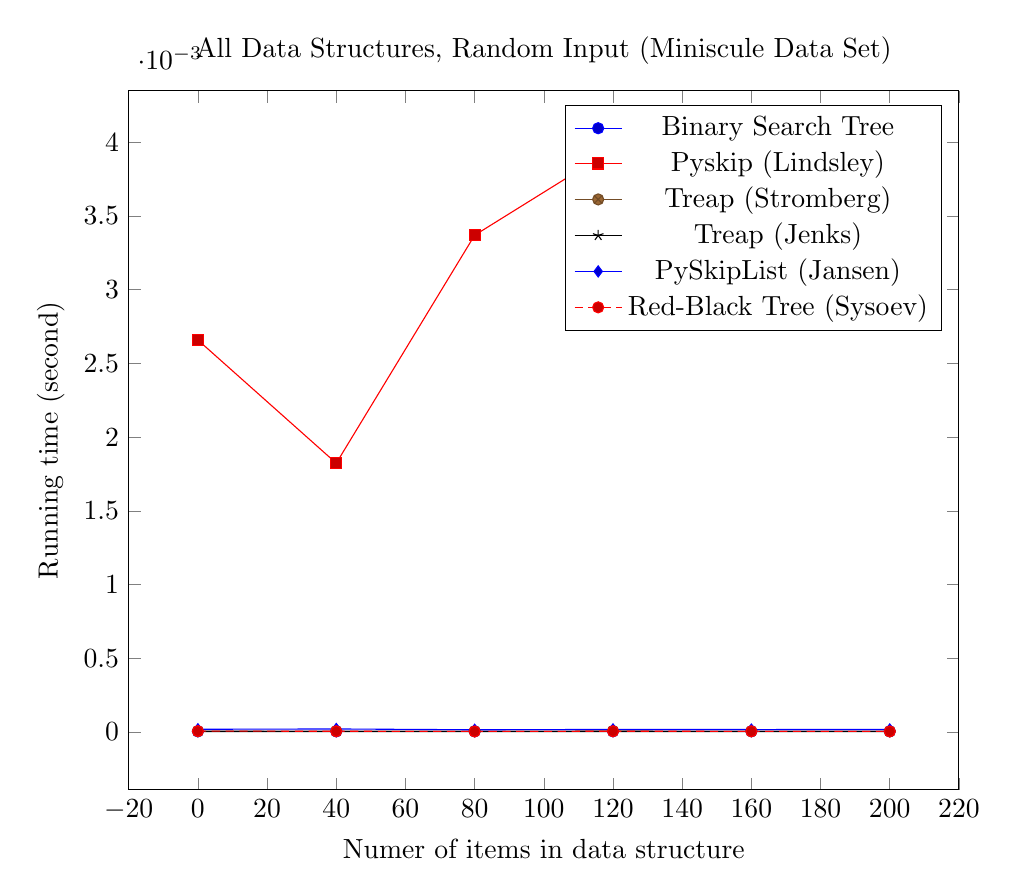
\begin{tikzpicture}
        \begin{axis}[
            xlabel={Numer of items in data structure},
            ylabel={Running time (second)},
            title={All Data Structures, Random Input (Miniscule Data Set)},
            width=\textwidth
        ]
		\addplot coordinates {
			(0, 3.945396911442245e-06)
			(40, 3.885161844097151e-06)
			(80, 4.035749512465436e-06)
			(120, 4.186337180844824e-06)
			(160, 4.487512517603598e-06)
			(200, 4.0658670461546365e-06)
		};
		\addplot coordinates {
			(0, 0.002658685520242754)
			(40, 0.0018228938432231722)
			(80, 0.003369429197443019)
			(120, 0.003953016647466734)
			(160, 0.0034237311106593447)
			(200, 0.002771716624125653)
		};
		\addplot coordinates {
			(0, 5.330803460501521e-06)
			(40, 6.113859336065453e-06)
			(80, 5.029628123742747e-06)
			(120, 6.655974942204601e-06)
			(160, 5.119980724765938e-06)
			(200, 4.4875125175813935e-06)
		};
		\addplot coordinates {
			(0, 3.2526936369237093e-06)
			(40, 2.349167626647386e-06)
			(80, 2.1383448909340075e-06)
			(120, 2.349167626647386e-06)
			(160, 2.1082273572448074e-06)
			(200, 2.198579958290203e-06)
		};
		\addplot coordinates {
			(0, 1.828134294081796e-05)
			(40, 2.0359452764417974e-05)
			(80, 1.490817916920406e-05)
			(120, 1.716699419485046e-05)
			(160, 1.6353820785619532e-05)
			(200, 1.6534525987665916e-05)
		};
		\addplot coordinates {
			(0, 5.812683999306678e-06)
			(40, 4.8790404553633595e-06)
			(80, 3.5839865073272747e-06)
			(120, 4.8489229217185684e-06)
			(160, 4.367042382913411e-06)
			(200, 3.734574175706662e-06)
		};
        \legend{Binary Search Tree, Pyskip (Lindsley), Treap (Stromberg), Treap (Jenks), PySkipList (Jansen), Red-Black Tree (Sysoev)}
        \end{axis}
    \end{tikzpicture}
    \caption{Average of 10 operations, benchmarked every 40, starting at 0.}
\end{figure}